\documentclass{ol-softwaremanual}

% Packages used in this example
\usepackage{graphicx}  % for including images
\usepackage{microtype} % for typographical enhancements
\usepackage{amsmath}   % for equations and mathematics
\usepackage{minted}    % for styled code blocks (requires -shell-escape + Pygments)
\usepackage{hyperref}  % for hyperlinks
\usepackage[a4paper,top=4.2cm,bottom=4.2cm,left=3.5cm,right=3.5cm]{geometry}

% Additional packages for lab content
\usepackage{enumitem}
\usepackage{changepage}  % for adjustwidth (wider code blocks)

% Code block style: light gray background, small monospace font, line wrapping
\setminted{style=friendly, bgcolor=gray!10, fontsize=\small, breaklines=true, breakanywhere=true}

% Wider code blocks: extend codemargin into each margin, normal text width unchanged
\newlength{\codemargin}
\setlength{\codemargin}{1.0cm}
\AddToHook{env/minted/before}{%
  \begin{adjustwidth}{-\codemargin}{-\codemargin}%
  \addtolength{\hsize}{2\codemargin}%
}
\AddToHook{env/minted/after}{\end{adjustwidth}}

% Give LaTeX extra inter-word stretch to avoid overfull boxes from long \texttt paths
\setlength{\emergencystretch}{2em}

% Custom macros used in this example document
\newcommand{\doclink}[2]{\href{#1}{#2}}
\newcommand{\cs}[1]{\texttt{\textbackslash #1}}

% Match original template cover spacing:
%   ~30% whitespace, logo, large gap, title+version, vfill, author+date
\makeatletter
\renewcommand\maketitle{%
  \begin{titlepage}
  \centering
  \vspace*{0.18\textheight}
  \@logocmd\par
  \vspace{0.10\textheight}
  {\huge\bfseries\@title\par}
  \bigskip
  {\Large\@ver\par}
  \vfill
  {\Large\@author\par}
  \@date
  \vspace{0.06\textheight}
  \end{titlepage}
}
\makeatother

% Frontmatter data; appears on title page
\title{Lab 1: ROS2 Introduction and System Integration}
\version{0.1.0}
\author{162 TAs and Maclab members}
\softwarelogo{
\includegraphics[width=8cm]{figures/capstone}}

\begin{document}

\maketitle

\centerline{\textbf{Warning!}}
\begin{itemize}
    \item No food and drinks are allowed in the lab.
    \item Be careful with the hardware especially the electronics.  Any liquid spill can cause a short circuit, potentially significantly delaying your progress.
    \item Never generate a short circuit.
    \item Connect electric wires only when you are sure about what you are doing.
    \item Be gentle to the buttons! You are liable to the damage made to the robot and its electronics.
    \item Wash your hands after each experiment, some components may contain some lead.
    \item Do not run experiments on the table for the chance the robot may fall on the floor and get damaged.
\end{itemize}
\pagebreak

\tableofcontents
\newpage

\section{System Architecture}

Figure~\ref{fig:system_architecture} shows the full system architecture of Project NUEVO.
The system is divided into several blocks that communicate over well-defined interfaces.
Understanding this structure is essential for debugging and extending the robot.
For a comprehensive reference covering all subsystems, see
\doclink{https://github.com/pochihh/Project-NUEVO/blob/main/docs/manual/MANUAL.md}{\texttt{docs/manual/MANUAL.md}}.

\begin{figure}[h]
  \centering
  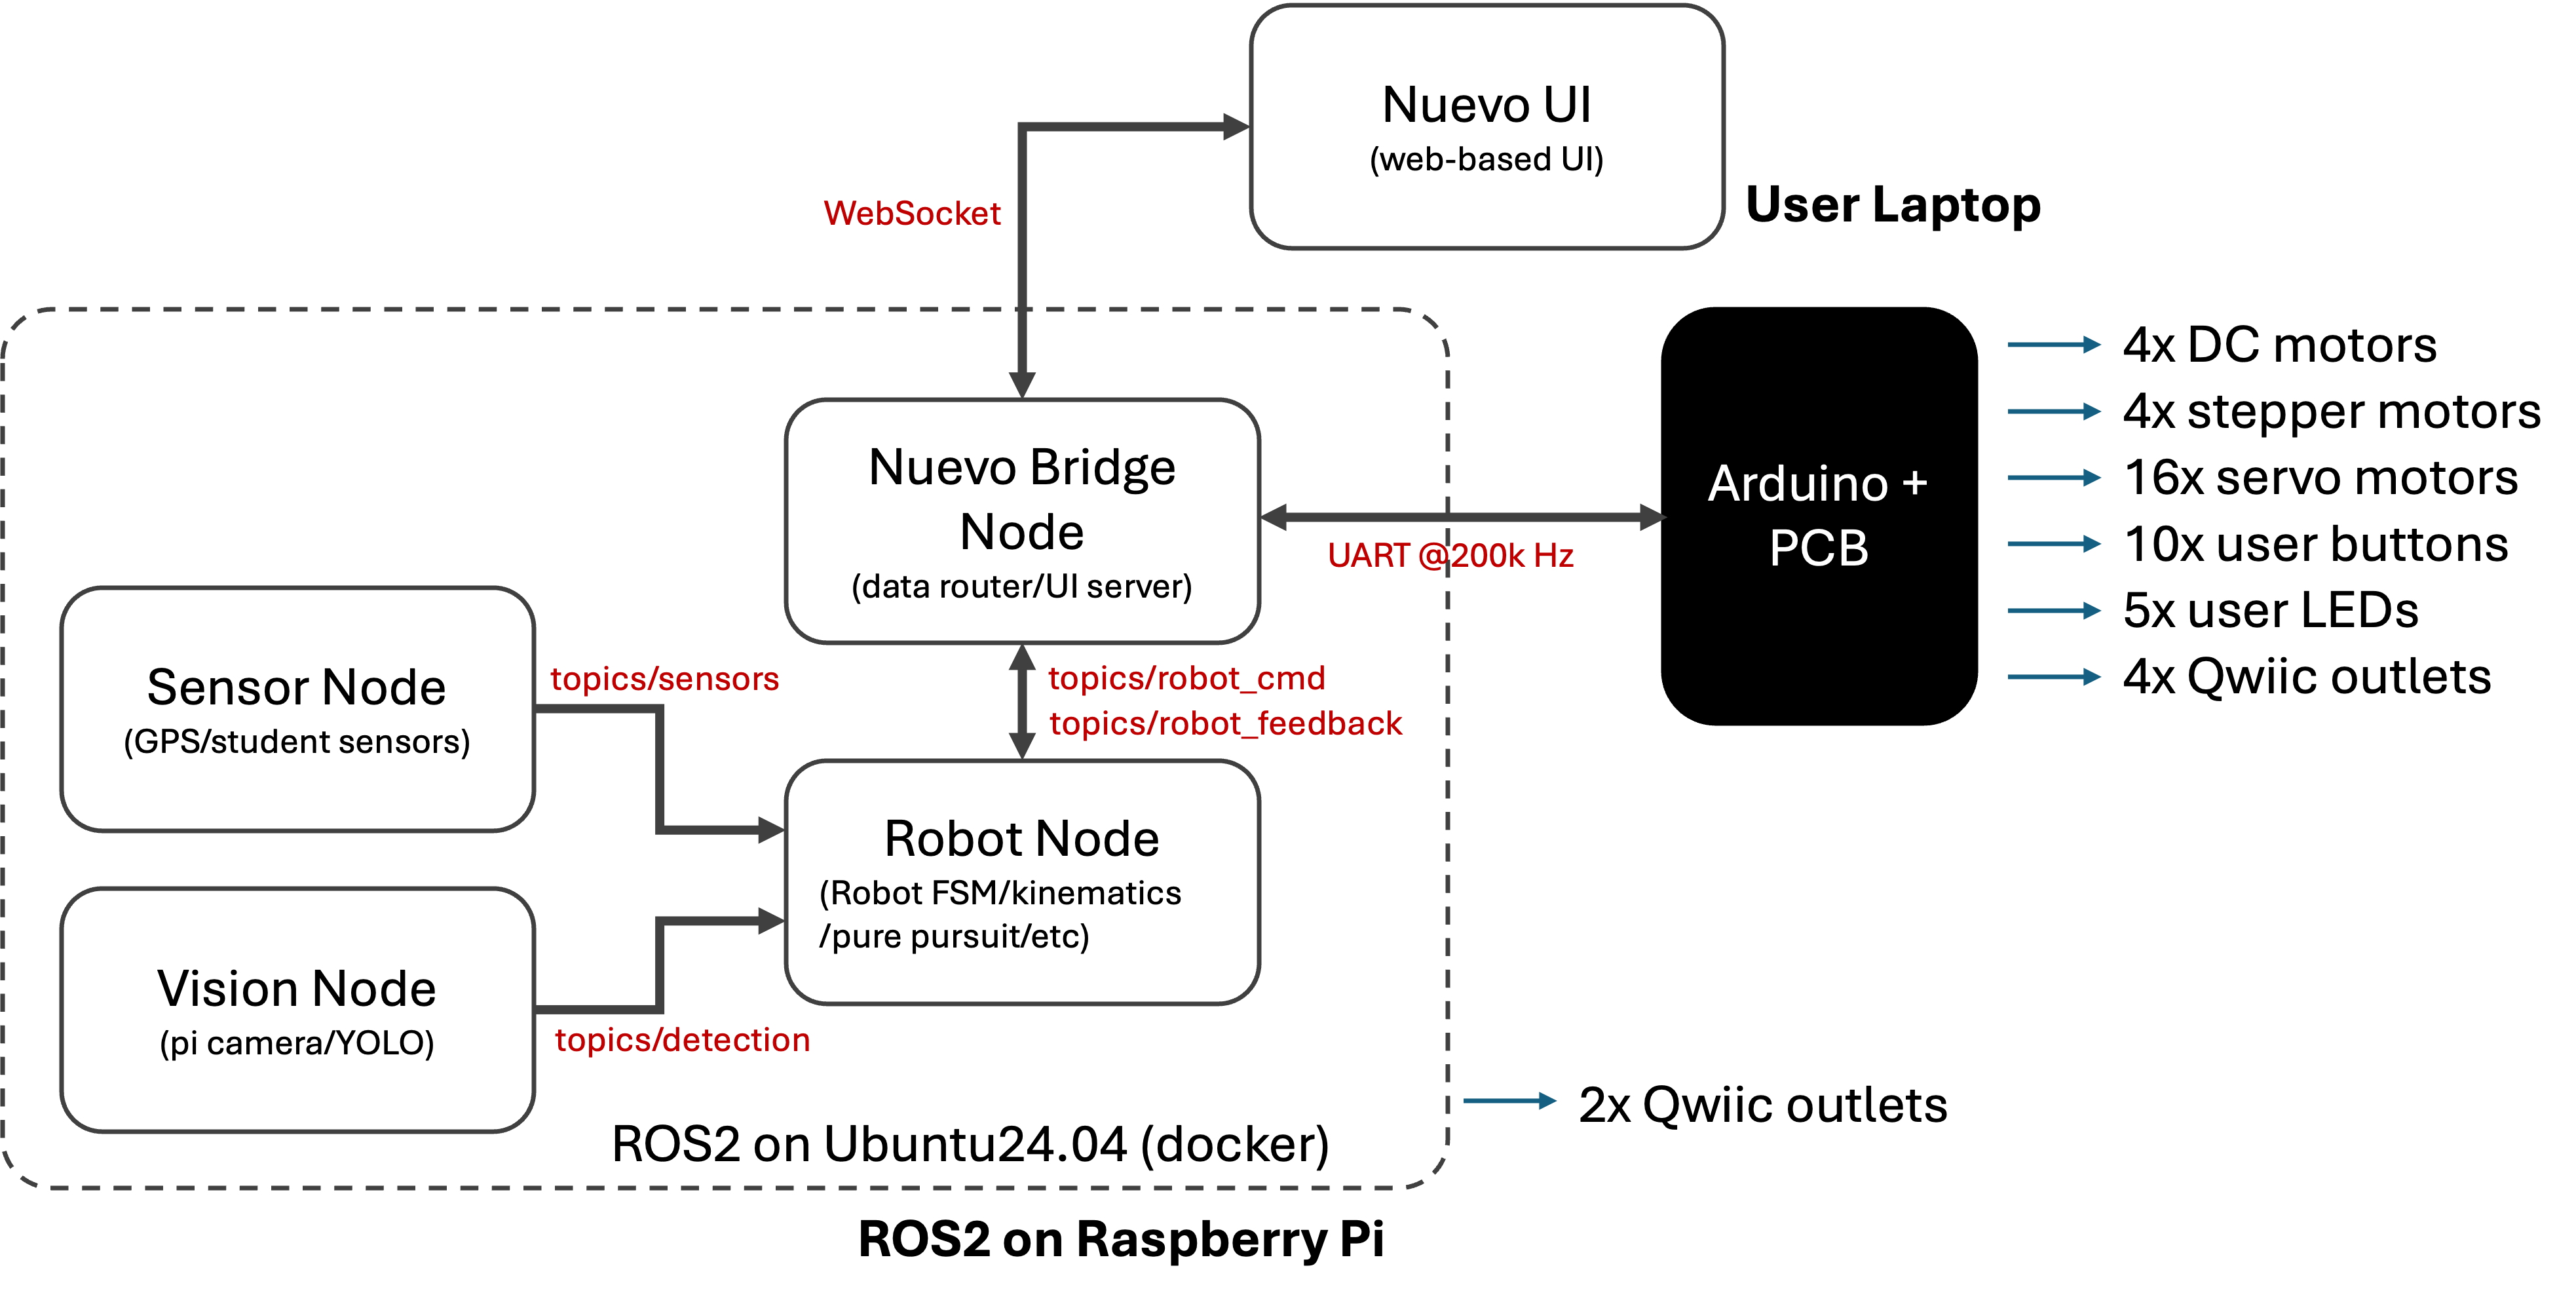
\includegraphics[width=\textwidth]{figures/system_architecture.png}
  \caption{System Architecture.}
  \label{fig:system_architecture}
\end{figure}

\subsection*{PCB and Firmware}
The custom PCB hosts an \textbf{Arduino Mega 2560} microcontroller and breaks out
the following hardware channels:

\begin{itemize}
  \item \textbf{4 DC motor channels} with quadrature encoder feedback
  \item \textbf{4 stepper motor channels} (A4988/DRV8825 drivers)
  \item \textbf{16 servo channels} via a PCA9685 I\textsuperscript{2}C PWM controller
  \item \textbf{IMU} (ICM-20948: accelerometer, gyroscope, magnetometer)
  \item \textbf{Voltage monitoring} for the battery rail, 5\,V rail, and servo rail
  \item \textbf{User I/O}: buttons, discrete LEDs, and NeoPixel RGB LEDs
  \item \textbf{Limit switches} and expandable ultrasonic sensor slots
\end{itemize}

The firmware runs hard real-time control loops: DC motor velocity control at 800\,Hz,
stepper pulse generation at 10\,kHz, and a soft scheduling loop at 100--200\,Hz for
UART communication and sensor reads.
The firmware is the only component that directly controls the actuators and reads
hardware encoders; all other layers communicate with it through the bridge.

For full firmware details refer to:
\begin{itemize}
  \item \doclink{https://github.com/pochihh/Project-NUEVO/blob/main/firmware/README.md}{\texttt{firmware/README.md}} --- build, upload, and configuration overview
  \item \doclink{https://github.com/pochihh/Project-NUEVO/blob/main/firmware/arduino/src/config.h}{\texttt{firmware/arduino/src/config.h}} --- all compile-time settings (channel counts, gains, rates)
  \item \doclink{https://github.com/pochihh/Project-NUEVO/blob/main/firmware/docs/architecture.md}{\texttt{firmware/docs/architecture.md}} --- runtime task structure and startup order
  \item \doclink{https://github.com/pochihh/Project-NUEVO/blob/main/docs/COMMUNICATION_PROTOCOL.md}{\texttt{docs/COMMUNICATION\_PROTOCOL.md}} --- TLV protocol, message catalog, and state machine
  \item \doclink{https://github.com/pochihh/Project-NUEVO/blob/main/tlv_protocol/TLV_Payloads.md}{\texttt{tlv\_protocol/TLV\_Payloads.md}} --- exact payload byte layouts and IDs
\end{itemize}

\subsection*{Bridge}
The bridge is a Python process running on the \textbf{Raspberry Pi~5}.
It owns the single UART connection to the Arduino (\texttt{/dev/ttyAMA0} at 200\,kbaud)
and translates between the compact TLV wire protocol and higher-level interfaces.
In addition to the transport layer, the bridge runs a \textbf{FastAPI/WebSocket server}
that serves the NUEVO web UI.
When running inside the ROS2 Docker container, the bridge also publishes and subscribes
to ROS2 topics and services, acting as the boundary between the real-time firmware world
and the robot application layer.

Refer to:
\begin{itemize}
  \item \doclink{https://github.com/pochihh/Project-NUEVO/blob/main/ros2_ws/BRIDGE_RUNTIME.md}{\texttt{ros2\_ws/BRIDGE\_RUNTIME.md}} --- bridge architecture, shared runtime model, and reset recovery
  \item \doclink{https://github.com/pochihh/Project-NUEVO/blob/main/docs/COMMUNICATION_PROTOCOL.md}{\texttt{docs/COMMUNICATION\_PROTOCOL.md}} --- TLV protocol, message catalog, and state machine
\end{itemize}

\subsection*{NUEVO UI}
The NUEVO UI is a \textbf{React} web application served by the bridge backend.
It provides a dashboard for testing and monitoring all hardware in real time:
motor speed setpoints and feedback, stepper positions, servo angles, LED color,
user button states, IMU readings, voltage levels, and odometry.
You access it from any browser on the same network by navigating to the
Raspberry Pi's IP address at port~8000.

Refer to:
\begin{itemize}
  \item \doclink{https://github.com/pochihh/Project-NUEVO/blob/main/ros2_ws/README.md}{\texttt{ros2\_ws/README.md}} --- build instructions for the frontend and how to start the bridge that serves the UI
\end{itemize}

\subsection*{Robot Node}
The \texttt{robot} ROS2 package is where high-level \textbf{decision-making and path planning}
code lives.
It subscribes to sensor and state topics published by the bridge, computes motion commands,
and publishes velocity setpoints back to the bridge for execution.
In this lab the robot node is a scaffold; you will extend it in future labs.

\subsection*{Sensor Node}
The \texttt{sensors} ROS2 package handles \textbf{Raspberry Pi--connected sensors}
that are not part of the Arduino firmware, such as GPS receivers and external range sensors
(LiDAR, ultrasonic modules, etc.).
It publishes sensor data as ROS2 topics for the robot node to consume.

\subsection*{Vision Node}
The \texttt{vision} ROS2 package handles the \textbf{camera pipeline and object detection}.
It reads frames from the camera, runs inference (e.g.\ YOLO), and publishes detection results
as ROS2 topics.
The vision dependencies (OpenCV, libcamera, YOLO) are heavier than the rest of the stack
and are added to the Docker image separately.

Refer to the following for the Robot, Sensor, and Vision nodes:
\begin{itemize}
  \item \doclink{https://github.com/pochihh/Project-NUEVO/blob/main/ros2_ws/ROS2_NODES_DESIGN.md}{\texttt{ros2\_ws/ROS2\_NODES\_DESIGN.md}} --- package layout, design principles, and topic/service naming
  \item \doclink{https://github.com/pochihh/Project-NUEVO/blob/main/ros2_ws/README.md}{\texttt{ros2\_ws/README.md}} --- Docker workflow, node startup order, and ROS2 API overview
\end{itemize}

\subsection*{Why ROS2 and Docker?}
With this architecture, each component has a single responsibility and communicates
through a standardised message-passing system.
Adding a new sensor, planner, or perception algorithm means writing a new node
that subscribes and publishes standard topics --- the rest of the system does not change.
Docker ensures that every team member and every Raspberry Pi runs the \emph{exact same}
software environment regardless of the host operating system, eliminating
``it works on my machine'' problems and making deployment to the robot a one-command step.


\section{ROS2 Introduction}

\subsection{Core Concepts}

ROS2 (Robot Operating System~2) is an open-source middleware framework for building
robot software.
Despite the name it is not an operating system: it is a set of libraries, tools, and
conventions that run on top of a standard OS and let independently developed programs
communicate with each other cleanly.

\textbf{Nodes} are the basic executable units.
Each node is a process (or a thread within a process) that performs one focused task ---
reading a sensor, running a controller, publishing odometry.
In this project: \texttt{bridge}, \texttt{robot}, \texttt{sensor\_node}, and
\texttt{vision\_node} are each a separate node.

\textbf{Topics} are named communication channels that carry a stream of messages.
A node that produces data \emph{publishes} to a topic; a node that needs that data
\emph{subscribes} to it.
Topics are asynchronous and many-to-many.
For example, the bridge node publishes DC motor state on \texttt{/dc\_state\_all}
and the robot node subscribes to that topic.

\textbf{Messages} define the data structure for a topic.
They are declared in \texttt{.msg} files inside the \texttt{bridge\_interfaces} package
and compiled into language-specific code automatically.
\texttt{bridge\_interfaces/msg/DCStateAll} and \texttt{bridge\_interfaces/msg/SystemPower}
are examples used in this project.

\textbf{Services} are synchronous request--reply interactions.
A node that handles a service advertises it; another node calls it and waits for
a response.
Use services for discrete operations where you need to know whether the action
succeeded.
In this project, firmware state transitions (IDLE $\to$ RUNNING, triggering an E-stop)
use the \texttt{/set\_firmware\_state} service.

\textbf{Packages} are the unit of organisation and distribution.
A package groups related nodes, message definitions, and launch files.
This project has five packages:
\texttt{bridge\_interfaces} (message/service definitions),
\texttt{bridge} (ROS wrapper around the firmware bridge),
\texttt{robot} (motion planning),
\texttt{sensors} (Pi-side sensors), and
\texttt{vision} (camera and detection).

\medskip
\noindent\textit{Keywords for further learning:}
ROS2 publisher/subscriber, colcon build, \texttt{ros2 topic echo}, \texttt{ros2 node info},
QoS policies, launch files, parameter server, tf2 transforms, RViz2, rqt.

\subsection{Docker for ROS2}

Modern robots are developed by teams working on different machines with different
operating systems --- macOS, Windows, Ubuntu.
ROS2 Jazzy officially targets Ubuntu 24.04; running it natively on macOS or Windows
requires significant manual setup that is fragile and hard to reproduce.
Docker solves this by packaging the entire ROS2 environment --- OS libraries,
ROS installation, workspace build --- into a single \emph{container image}.
Everyone on the team starts the same image, so the software environment is
\emph{identical} whether you are developing on a laptop or deploying to the Raspberry Pi.
This also means updating the environment is a \texttt{docker compose build} rather than
a multi-step manual procedure.

In this project the Docker image contains ROS2 Jazzy, the project workspace,
and all Python runtime dependencies.
Two compose files are provided:

\begin{itemize}
  \item \texttt{ros2\_ws/docker/docker-compose.rpi.yml} --- for the Raspberry Pi with real hardware
  \item \texttt{ros2\_ws/docker/docker-compose.vm.yml} --- for macOS / Windows development (mock bridge)
\end{itemize}

\noindent\textit{Keywords for further learning:}
Dockerfile, Docker image vs.\ container, \texttt{docker compose}, volume mounts,
container networking, \texttt{docker exec}, base images.


\section{Lab Activities}

\subsection{Task 1: Set Up Your Repository}

In this course you will modify the Project NUEVO codebase to add features and
tune your robot.
Each team should work in their own copy of the repository so that your changes
do not affect other teams and so you can safely experiment.

\subsubsection*{1.1 Fork the Repository}

\begin{enumerate}
  \item Go to \doclink{https://github.com/pochihh/Project-NUEVO}{github.com/pochihh/Project-NUEVO}.
  \item Click \textbf{Fork} (top-right corner) to create a copy under your own GitHub account.
    \hfill\textit{(keyword: fork)}
  \item On your forked repository page, go to \textbf{Settings $\to$ Collaborators}
        and add your teammates as collaborators so everyone can push to the same fork.
    \hfill\textit{(keyword: collaborators, repository permissions)}
\end{enumerate}

\subsubsection*{1.2 Clone and Collaborate with Git}

Git lets your whole team work on the same codebase simultaneously.
The basic workflow is:

\begin{enumerate}
  \item \textbf{Clone} your fork to your local machine.
        This downloads the full repository history.
\begin{minted}{bash}
git clone https://github.com/<your-username>/Project-NUEVO.git
cd Project-NUEVO
\end{minted}
        \hfill\textit{(keyword: clone, remote)}

  \item \textbf{Make changes}, then \textbf{stage} the files you want to save.
\begin{minted}{bash}
git add <filename>
\end{minted}
        \hfill\textit{(keyword: staging area, working tree)}

  \item \textbf{Commit} to record a snapshot with a short message describing what you did.
\begin{minted}{bash}
git commit -m "brief description of change"
\end{minted}
        \hfill\textit{(keyword: commit, commit message)}

  \item \textbf{Push} to upload your commits to GitHub so teammates can see them.
\begin{minted}{bash}
git push
\end{minted}
        \hfill\textit{(keyword: push, origin)}

  \item \textbf{Pull} to download your teammates' latest commits before you start working.
\begin{minted}{bash}
git pull
\end{minted}
        \hfill\textit{(keyword: pull, merge, rebase, merge conflict)}
\end{enumerate}

\subsubsection*{1.3 Pull Updates from the Original Repository}

Bug fixes and new features will be released to the original repository during the
course.
To bring them into your fork, add the original repository as a second remote and
pull from it:

\begin{enumerate}
  \item Add the original repository as the \texttt{upstream} remote (one-time setup):
\begin{minted}{bash}
git remote add upstream https://github.com/pochihh/Project-NUEVO.git
\end{minted}
        \hfill\textit{(keyword: remote, upstream)}

  \item Fetch and merge the latest changes from upstream into your local branch:
\begin{minted}{bash}
git fetch upstream
git merge upstream/main
\end{minted}
        \hfill\textit{(keyword: fetch, merge, fast-forward)}

  \item Push the result to your fork:
\begin{minted}{bash}
git push
\end{minted}
\end{enumerate}


\subsection{Task 2: Flash the Firmware}

The Arduino Mega firmware must be flashed onto the robot before the bridge can
communicate with it.
Full details and troubleshooting are in
\doclink{https://github.com/pochihh/Project-NUEVO/blob/main/firmware/README.md}{\texttt{firmware/\allowbreak README.md}}.

\subsubsection*{2.1 Prerequisites}

\begin{enumerate}
  \item Install \textbf{Arduino IDE 2.x} and the \textbf{Arduino AVR Boards} core.
  \item Increase the serial buffer size so the firmware UART link does not overflow.
        Create or edit \texttt{platform.local.txt} for the installed AVR core and add:
\begin{minted}{text}
compiler.cpp.extra_flags=-DSERIAL_RX_BUFFER_SIZE=512 -DSERIAL_TX_BUFFER_SIZE=256
\end{minted}
        Typical file locations (replace \texttt{1.8.7} with your installed AVR core version):

        \textit{macOS:}
\begin{minted}{text}
~/Library/Arduino15/packages/arduino/hardware/avr/1.8.7/platform.local.txt
\end{minted}
        \textit{Windows:}
\begin{minted}{text}
C:\Users\<your-user>\AppData\Local\Arduino15\packages\arduino\hardware\avr\1.8.7\platform.local.txt
\end{minted}
\end{enumerate}

\subsubsection*{2.2 Build and Upload}

\begin{enumerate}
  \item Open \texttt{firmware/arduino/arduino.ino} in Arduino IDE.
  \item Select board: \textbf{Arduino Mega or Mega~2560}.
  \item Select the correct COM / serial port for the connected Arduino.
  \item Click \textbf{Verify} to confirm the firmware compiles without errors.
  \item Click \textbf{Upload} to flash the firmware onto the board.
\end{enumerate}

After a successful upload the board resets and the firmware starts running.
Confirm by opening the Arduino IDE Serial Monitor at 115\,200 baud and checking
for heartbeat output.


\subsection{Task 3: Bring Up the ROS2 Environment and NUEVO UI}

In this task you will start the Docker container on the Raspberry Pi, launch the
bridge node, and verify all hardware using the NUEVO web UI.
Full setup details are in
\doclink{https://github.com/pochihh/Project-NUEVO/blob/main/ros2_ws/README.md}{\texttt{ros2\_ws/README.md}}.

\subsubsection*{3.1 Raspberry Pi UART Setup (one-time)}

The bridge communicates with the Arduino over the RPi hardware UART.
Enable it by editing the RPi boot configuration files:

\begin{enumerate}
  \item Add the following lines to \texttt{/boot/firmware/config.txt}:
\begin{minted}{text}
enable_uart=1
dtoverlay=uart0-pi5
\end{minted}

  \item Remove any \texttt{console=serial0} or \texttt{console=ttyAMA0} entries
        from \texttt{/boot/firmware/cmdline.txt} so the OS does not claim the port.

  \item Reboot and verify: \texttt{ls -l /dev/ttyAMA0} should show a character
        device owned by the \texttt{dialout} group.
\end{enumerate}

\subsubsection*{3.2 Build the Frontend (one-time)}

The bridge serves the NUEVO web UI as a pre-built static bundle.
Build it once from the repository root:

\begin{minted}{bash}
cd nuevo_ui/frontend
npm install
npm run build
cd ../..
cp -r nuevo_ui/frontend/dist/. nuevo_ui/backend/static/
\end{minted}

\subsubsection*{3.3 Start the Docker Container}

From the repository root on the Raspberry Pi:

\begin{minted}{bash}
COMPOSE=ros2_ws/docker/docker-compose.rpi.yml
docker compose -f $COMPOSE build
docker compose -f $COMPOSE up -d
docker compose -f $COMPOSE logs -f ros2_runtime
\end{minted}

Wait until the log shows that \texttt{colcon build} finished and the container is ready.

\subsubsection*{3.4 Launch the Bridge Node}

Open a shell inside the running container and start the bridge:

\begin{minted}{bash}
docker compose -f $COMPOSE exec ros2_runtime bash
source /opt/ros/jazzy/setup.bash
source /ros2_ws/install/setup.bash
ros2 run bridge bridge
\end{minted}

The bridge node connects to the Arduino, starts the WebSocket server, and begins
publishing ROS2 topics.

\subsubsection*{3.5 Access the NUEVO UI}

Open a browser on any device on the same network and navigate to:
\begin{center}
  \texttt{http://<raspberry-pi-ip>:8000}
\end{center}

Login credentials: username \texttt{user}, password \texttt{162}.
\textbf{Change your password after first login.}

Use the UI to test each hardware feature:
\begin{itemize}
  \item Set stepper motor positions and verify movement.
  \item Command servo angles and observe the mechanical response.
  \item Change LED colors via the colour picker.
  \item Press each user button and confirm the indicator updates.
  \item Check IMU readings (accelerometer, gyroscope) for expected values.
  \item Monitor the battery voltage level on the power panel.
\end{itemize}


\subsection{Task 4: DC Motor PI Tuning and Step Response}

In this task you will tune the PI velocity controller for one DC motor and record
step responses to evaluate your design.
The goal is to transition from the default gains to a set of gains that you can
justify from a simple model of the motor dynamics.

\subsubsection*{4.1 Model-Based PI Design (Optional)}

A DC motor's velocity dynamics can be approximated as a first-order linear system:
\begin{equation}
  G(s) = \frac{K}{\tau s + 1}
  \label{eq:motor_model}
\end{equation}
where $K$ is the steady-state gain (ticks/s per PWM unit) and $\tau$ is the time
constant (seconds).
You can identify both parameters from an open-loop step response.

\paragraph{Step 1: Measure the open-loop step response.}
In the NUEVO UI, switch the motor to \textbf{PWM mode} and apply a step change in
PWM from 0 to a fixed value (e.g.\ 50\,\%).
Record the velocity $\omega(t)$ response using the UI's plot feature.

From the recorded curve:
\begin{itemize}
  \item $K = \omega_{ss} / u$ \quad (steady-state velocity divided by the applied PWM)
  \item $\tau$ = the time at which $\omega(t)$ first reaches $63.2\,\%$ of $\omega_{ss}$
\end{itemize}

\paragraph{Step 2: Choose the closed-loop bandwidth.}
A PI controller with plant $G(s)$ gives a second-order closed-loop response.
Matching coefficients to the standard form $s^2 + 2\zeta\omega_n s + \omega_n^2$:
\begin{equation}
  K_p = \frac{2\zeta\omega_n\tau - 1}{K}, \qquad
  K_i = \frac{\omega_n^2 \,\tau}{K}
  \label{eq:pi_gains}
\end{equation}

Choose a desired damping ratio $\zeta = 0.7$ (a good default that balances speed and
overshoot).
Select $\omega_n$ based on a rise-time or settling-time specification of your choice,
then compute $K_p$ and $K_i$ from Equations~\eqref{eq:pi_gains}.

\subsubsection*{4.2 Simple Observation (Alternative to 4.1)}

If you prefer a faster approach, skip the model identification and instead adjust
$K_p$ and $K_i$ manually while observing the step response:
increase $K_p$ to speed up the response, increase $K_i$ to eliminate steady-state
error, and reduce both if the response oscillates.

\subsubsection*{4.3 Record and Compare Step Responses}

Using the NUEVO UI, command a velocity step from 0 to 1000 ticks/s and record the
response for:
\begin{enumerate}
  \item The \textbf{default} PI gains (as shipped in \texttt{firmware/\allowbreak arduino/\allowbreak src/\allowbreak config.h}).
  \item Your \textbf{tuned} gains from Task~4.1 or~4.2.
\end{enumerate}

On each plot, annotate:
\begin{itemize}
  \item Rise time $t_r$ (time to go from 10\,\% to 90\,\% of the setpoint)
  \item Percent overshoot $M_p$
  \item Settling time $t_s$ (time to stay within $\pm 5\,\%$ of the setpoint)
  \item Steady-state error $e_{ss}$
\end{itemize}

A MATLAB script (\texttt{plot\_step\_response.m}) is provided in the lab repository to load the exported CSV, compute all four metrics automatically, and produce an annotated plot.
Figure~\ref{fig:example_step} shows an example output.

\begin{figure}[h]
  \centering
  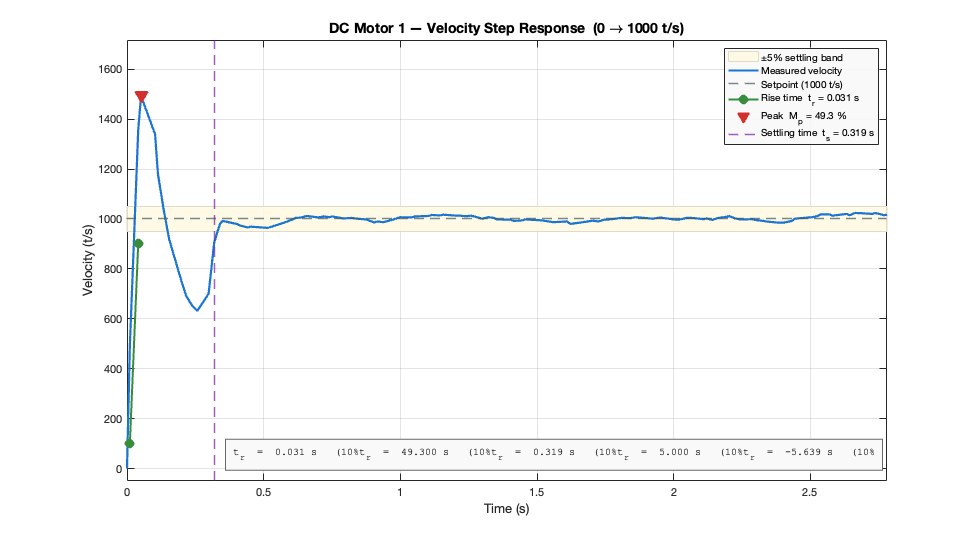
\includegraphics[width=\textwidth]{figures/example_step.png}
  \caption{Example annotated velocity step response (0 $\to$ 1000\,ticks/s).
           The shaded region is the $\pm5\,\%$ settling band.}
  \label{fig:example_step}
\end{figure}


\section{Lab Deliverables}

Show your final step response plots to the TAs.
Your plots should include both the default and tuned step responses with the
performance metrics annotated.
Justify your tuned gains: explain how you arrived at your $K_p$ and $K_i$ values,
whether through the model-based approach or manual tuning, and discuss the
trade-offs you observed between rise time, overshoot, and settling time.

\end{document}
